\documentclass{standalone}
\usepackage{tikz}
\usepackage{ctex,siunitx}
\usepackage{tkz-euclide}
\usepackage{amsmath}
\usetikzlibrary{patterns, calc}
\usetikzlibrary {decorations.pathmorphing, decorations.pathreplacing, decorations.shapes,}
\begin{document}
\small
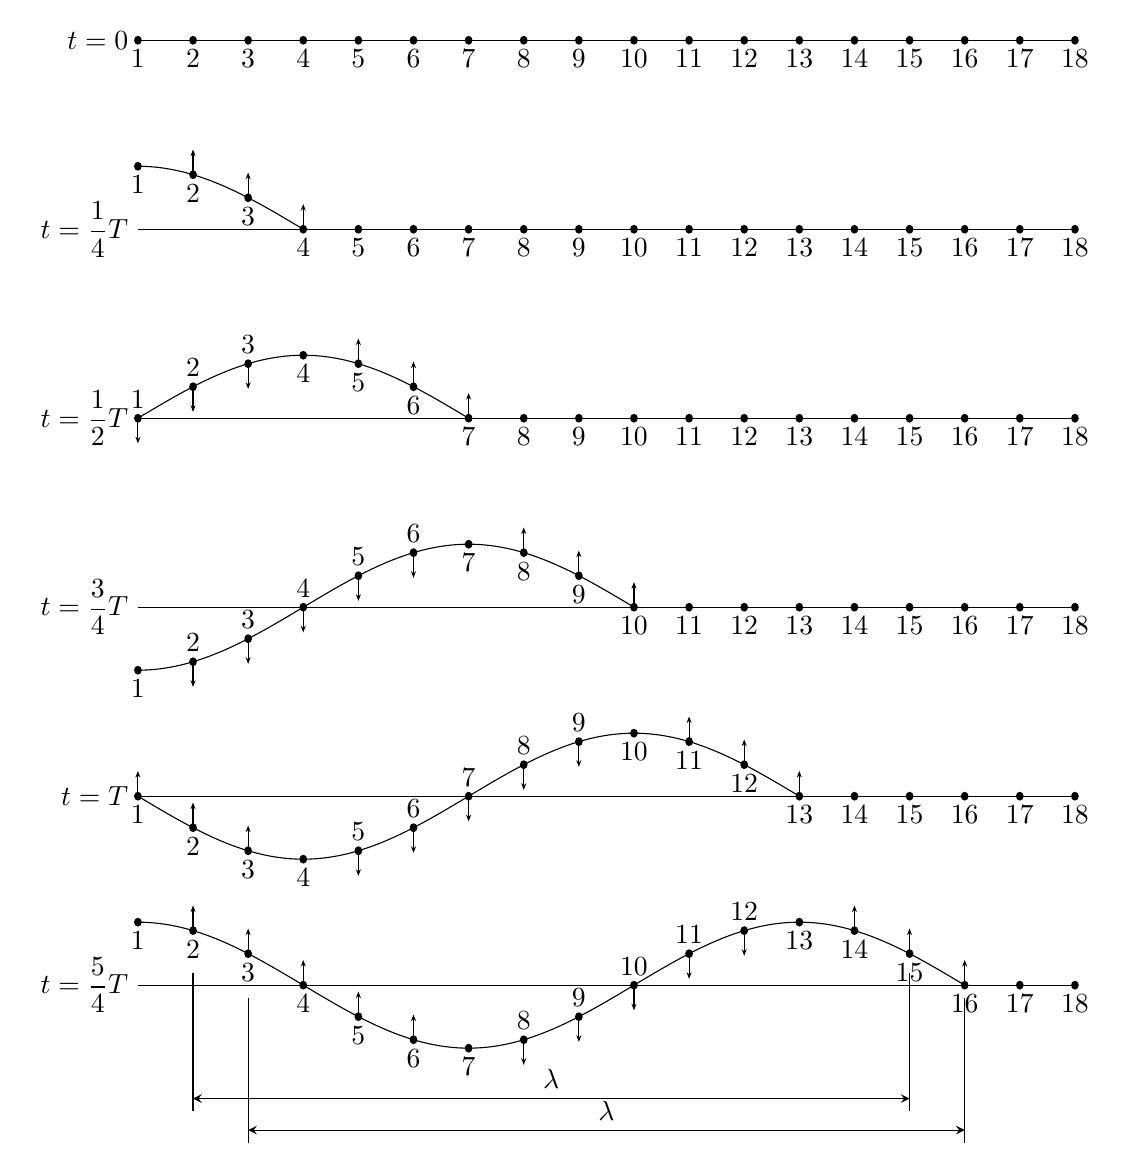
\begin{tikzpicture}[>=stealth,xscale=0.7,yscale=0.8,samples=200]
  \useasboundingbox(-2.0,0.2)rectangle(17.5,-17.5);
  \draw (0,0)--(17,0) node [at start,left]{$t=0$};
  \foreach \x[count=\i] in {0,1,...,17} {\fill(\x,0)circle(2pt)node[below]{\i};}
  \begin{scope}[yshift=-3cm]
    \draw [domain=0:3]  plot (\x,{cos(1/6*pi*\x r)});
    \draw (0,0)--(17,0) node [at start,left]{$t=\dfrac{1}{4}T$};
    \foreach \x in {0,1,2,3} { \fill(\x,{cos(1/6*pi*\x r)})circle(2pt); }
    \foreach \x[count=\i from 2] in {1,2,3} 
      { 
        \draw[arrows={-Stealth[scale=0.5]}](\x,{cos(1/6*pi*\x r)})--++(0,0.4)node[at start,below]{\i}; 
      }
    \foreach \x[count=\i from 5] in {4,5,...,17} {\fill(\x,0)circle(2pt)node[below]{\i};}
    \foreach \x[count=\i] in {0} {\node at (\x,{cos(1/6*pi*\x r)})[below]{\i};}
  \end{scope}
  \begin{scope}[yshift=-6cm]
    \draw [domain=0:6]  plot (\x,{sin(1/6*pi*\x r)});
    \draw (0,0)--(17,0)node [at start,left]{$t=\dfrac{1}{2}T$};
    \foreach \x in {0,1,...,6}
    {
      \fill(\x,{sin(1/6*pi*\x r)})circle(2pt);
    }
    \foreach \x[count=\i from 5] in {4,5,6} 
      { 
        \draw[arrows={-Stealth[scale=0.5]}](\x,{sin(1/6*pi*\x r)})--++(0,0.4)node[at start,below]{\i}; 
      }
    \foreach \x[count=\i] in {0,1,2} 
      { 
        \draw[arrows={-Stealth[scale=0.5]}](\x,{sin(1/6*pi*\x r)})--++(0,-0.4)node[at start,above]{\i}; 
      }
    \foreach \x[count=\i from 8] in {7,8,...,17} {\fill(\x,0)circle(2pt)node[below]{\i};}
    \foreach \x/\y in {3/4} {\node at (\x,{sin(1/6*pi*\x r)})[below]{\y};}
  \end{scope}
  \begin{scope}[yshift=-9cm]
    \draw [domain=0:9]  plot (\x,{-cos(1/6*pi*\x r)});
    \draw (0,0)--(17,0)node [at start,left]{$t=\dfrac{3}{4}T$};
    \foreach \x in {0,1,...,9}
    {
      \fill(\x,{-cos(1/6*pi*\x r)})circle(2pt);
    }
    \foreach \x[count=\i from 2] in {1,2,...,5} 
      { 
        \draw[arrows={-Stealth[scale=0.5]}](\x,{-cos(1/6*pi*\x r)})--++(0,-0.4)node[at start,above]{\i}; 
      }
    \foreach \x[count=\i from 8] in {7,8,...,9} 
      { 
        \draw[arrows={-Stealth[scale=0.5]}](\x,{-cos(1/6*pi*\x r)})--++(0,0.4)node[at start,below]{\i}; 
      }
    \foreach \x/\y in {0/1,6/7} {\node at (\x,{-cos(1/6*pi*\x r)})[below]{\y};}
    \foreach \x[count=\i from 11] in {10,11,...,17} {\fill(\x,0)circle(2pt)node[below]{\i};}
  \end{scope}
  \begin{scope}[yshift=-12cm]
    \draw [domain=0:12]  plot (\x,{-sin(1/6*pi*\x r)});
    \draw (0,0)--(17,0)node [at start,left]{$t=T$};
    \foreach \x in {0,1,...,12} { \fill(\x,{-sin(1/6*pi*\x r)})circle(2pt); }
    \foreach \x[count=\i from 5] in {4,5,...,8} 
      { 
        \draw[arrows={-Stealth[scale=0.5]}](\x,{-sin(1/6*pi*\x r)})--++(0,-0.4)node[at start,above]{\i}; 
      }
    \foreach \x[count=\i from 11] in {10,11,12} 
      { 
        \draw[arrows={-Stealth[scale=0.5]}](\x,{-sin(1/6*pi*\x r)})--++(0,0.4)node[at start,below]{\i}; 
      }
    \foreach \x[count=\i from 1] in {0,1,2} 
      { 
        \draw[arrows={-Stealth[scale=0.5]}](\x,{-sin(1/6*pi*\x r)})--++(0,0.4)node[at start,below]{\i}; 
      }
    \foreach \x[count=\i from 14] in {13,14,...,17} {\fill(\x,0)circle(2pt)node[below]{\i};}
    \foreach \x/\y in {3/4,9/10} {\node at (\x,{-sin(1/6*pi*\x r)})[below]{\y};}
  \end{scope}
  \begin{scope}[yshift=-15cm]
    \draw [domain=0:15]  plot (\x,{cos(1/6*pi*\x r)});
    \draw (0,0)--(17,0)node [at start,left]{$t=\dfrac{5}{4}T$};
    \foreach \x in {0,1,...,15}
    {
      \fill(\x,{cos(1/6*pi*\x r)})circle(2pt);
    }
    \foreach \x[count=\i from 2] in {1,2,...,5} 
      { 
        \draw[arrows={-Stealth[scale=0.5]}](\x,{cos(1/6*pi*\x r)})--++(0,0.4)node[at start,below]{\i}; 
      }
    \foreach \x[count=\i from 14] in {13,14,...,15} 
      { 
        \draw[arrows={-Stealth[scale=0.5]}](\x,{cos(1/6*pi*\x r)})--++(0,0.4)node[at start,below]{\i}; 
      }
    \foreach \x[count=\i from 8] in {7,8,...,11} 
      { 
        \draw[arrows={-Stealth[scale=0.5]}](\x,{cos(1/6*pi*\x r)})--++(0,-0.4)node[at start,above]{\i}; 
      }
    \foreach \x[count=\i from 17] in {16,17} {\fill(\x,0)circle(2pt)node[below]{\i};}
    \foreach \x/\y in {0/1,6/7,12/13} {\node at (\x,{cos(1/6*pi*\x r)})[below]{\y};}
    \draw[thin] (1,0.2)--(1,-2)(14,0.2)--(14,-2);
    \draw[thin,<->](1,-1.8)--(14,-1.8)node[midway,above]{$\lambda$};
    \draw[thin] (2,-0.2)--(2,-2.5)(15,-0.2)--(15,-2.5);
    \draw[thin,<->](2,-2.3)--(15,-2.3)node[midway,above]{$\lambda$};
  \end{scope}

  % \draw [double=brown!80!black,double distance=1pt, domain=0.5*pi:1.5*pi]  plot (\x,{0.5*cos(2*\x r)});
  % \draw [double=brown!80!black,double distance=1pt, domain=1.5*pi:2.5*pi]  plot (\x,-0.5);
  % \draw [double=brown!80!black,double distance=1pt, domain=2.5*pi:3.5*pi]  plot (\x,{0.3*cos(2*\x r)-0.2});
  % \draw [double=brown!80!black,double distance=1pt, domain=3.5*pi:12]  plot (\x,-0.5);
  % \draw[thin,->](pi,0.6)--++(0.5,0)node[right]{1};
  % \draw[thin,->](3*pi,0.4)--++(-0.5,0)node[left]{2};
\end{tikzpicture}
\end{document}